\section{Description de l'utilisation du jeu}
Pour pouvoir rester au plus proche du jeu original, nous avons utilisé des bases de données créées par les fans sur le site de Pokémon essentials. Nous en avons extrait divers éléments graphiques ainsi que des polices de caractère et des fichiers contenant de vraies données sur les Pokémon. C'est pourquoi notre  interface graphique et celle du vrai jeu se ressemblent beaucoup. 

\subsection{Présentation de l'interface de combat}
\begin{figure}[!h]
\begin{minipage}{0.49\textwidth}
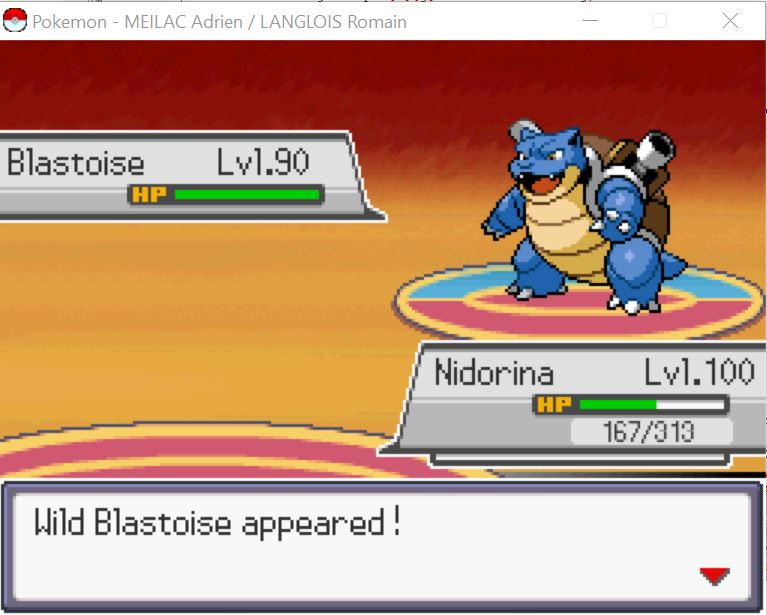
\includegraphics[scale = 0.6]{../Images/combat_start.jpg}
\end{minipage}
\begin{minipage}{0.49\textwidth}
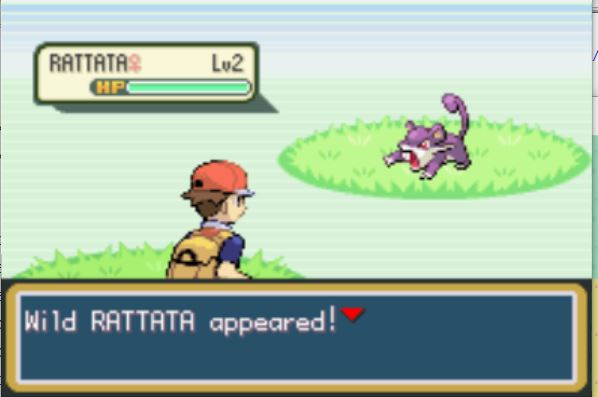
\includegraphics[scale = 0.84]{../Images/vrai_jeu_combat_start.jpg}
\end{minipage}
\caption{Début de combat}
\end{figure}

Prenons par exemple la rencontre d'un pokémon aléatoire, générée par une loi binomiale lors du déplacement sur la carte. Une fenêtre de dialogue va apparaître, ainsi que l'arrière-plan de combat et également le Pokémon ennemi. Une pression de la touche entrée permet alors d'afficher le menu contextuel de combat.

\begin{figure}[!h]
\begin{minipage}{0.49\textwidth}
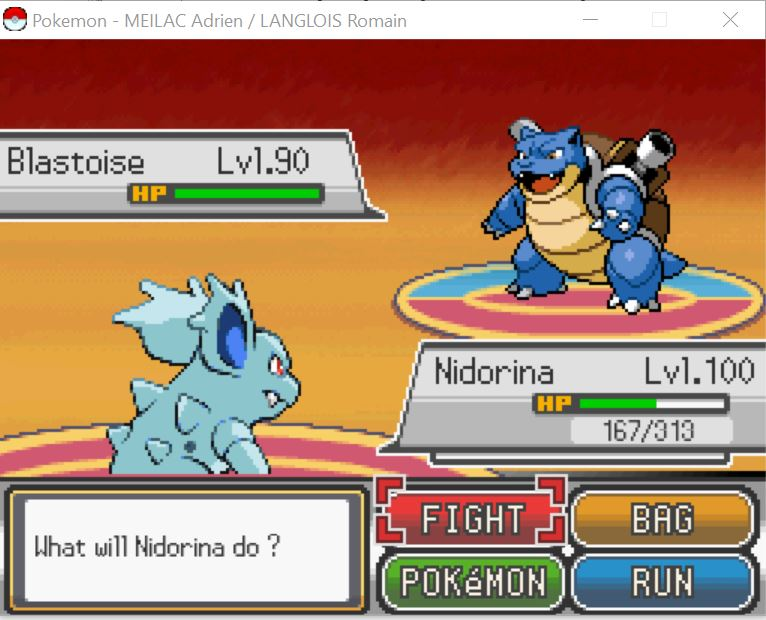
\includegraphics[scale = 0.6]{../Images/mainMenu.jpg}
\end{minipage}
\begin{minipage}{0.49\textwidth}
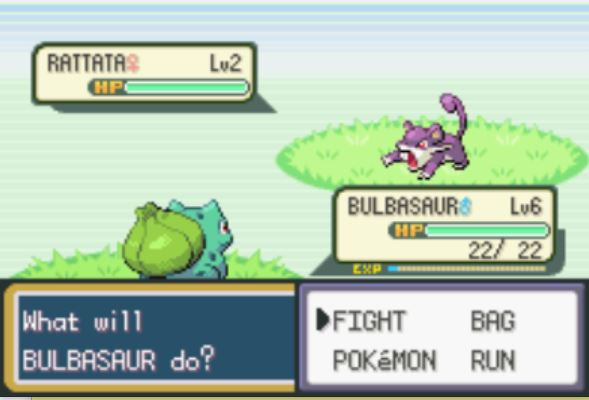
\includegraphics[scale = 0.84]{../Images/vrai_jeu_mainMenu.jpg}
\end{minipage}
\caption{Menu principal}
\end{figure}


Dans ce menu, comme dans le jeu original, le joueur a le choix entre accéder à son inventaire (BAG), choisir son pokémon destiné à combattre (POKEMON), s'enfuir (RUN), ou alors attaquer (FIGHT).

Si le joueur décide de s'enfuir, il revient sur la map générale et ses Pokemon gardent les dégâts qu'ils ont subis lors du combat. Cependant, nous n'avons pas eu le temps de conserver la position du joueur lors du lancement du combat, c'est pourquoi ce dernier est remis à sa position initiale. 

\begin{figure}[!h]
\begin{minipage}{0.49\textwidth}
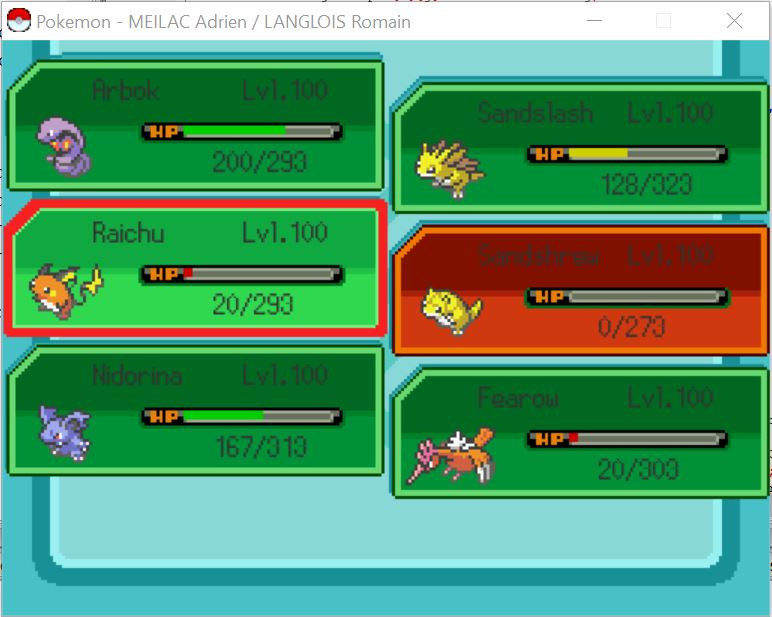
\includegraphics[scale = 0.6]{../Images/swapMenu.jpg}
\end{minipage}
\begin{minipage}{0.49\textwidth}
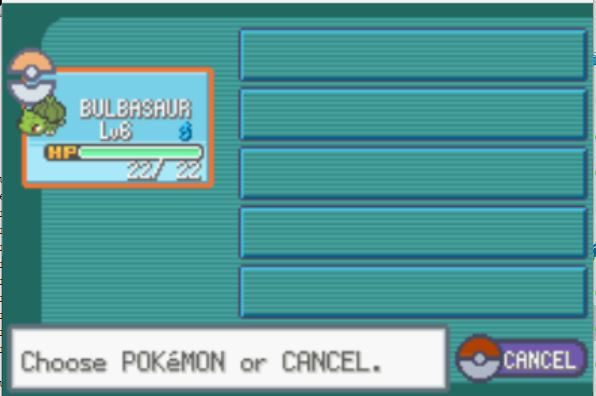
\includegraphics[scale = 0.84]{../Images/vrai_jeu_swapMenu.jpg}
\end{minipage}
\caption{Menu du dresseur}
\end{figure}

Le menu Pokemon, appelé menu du dresseur, permet au joueur de choisir le Pokemon qui va combattre, et de voir l'état de santé ainsi que le niveau de ses Pokemon. Les Pokemon morts apparaissent en rouge et ne peuvent être sélectionnés pour combattre. 

Nous avons réalisé un effet visuel sur les barres d'HP. Leur longueur est ainsi adaptée au pourcentage de leur vie restant, et la couleur change: rouge en-dessous de 20\%, orange entre 20 et 50\%, et vert au-delà. Cet effet est aussi visible sur l'écran de combat principal, ce qui rend le combat plus interactif. 

\begin{figure}[!h]
\begin{minipage}{0.49\textwidth}
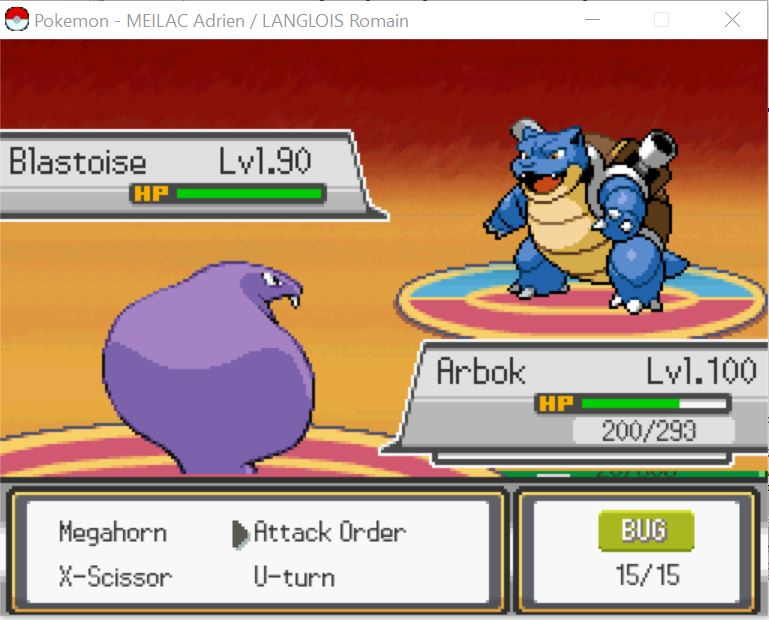
\includegraphics[scale = 0.6]{../Images/fightMenu.jpg}
\end{minipage}
\begin{minipage}{0.49\textwidth}
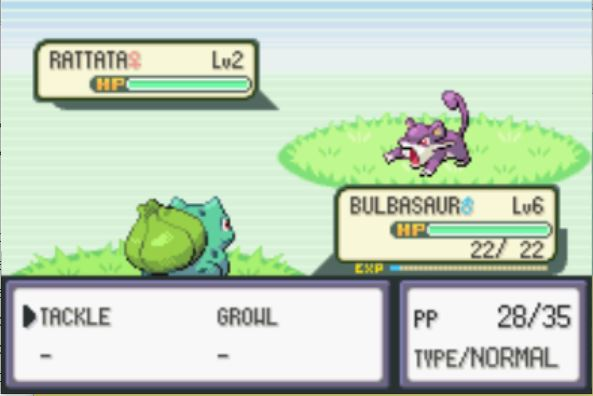
\includegraphics[scale = 0.84]{../Images/vrai_jeu_fightMenu.jpg}
\end{minipage}
\caption{Menu de combat}
\end{figure}


Si le combat est adopté, un menu comprenant les diverses capacités disponibles pour le Pokemon retenu apparaît. Lorsque le joueur sélectionne une capacité à l'aide du curseur, il peut voir son type ainsi que ses Points de puissance (PP). Le combat se déroule ensuite au tour par tour en respectant les priorités d'ordre d'attaque entre les Pokemon. A chaque étape le menu est remplacé par une fenêtre de dialogue indiquant l'attaque utilisée. On voit alors le Pokemon touché perdre ses points de vie progressivement. Certaines capacités, comme Hail (Grêle dans le jeu français) de Nidorina, ne font pas de dégâts à l'adversaire mais ont un effet sur le temps du terrain, qui va se répercuter durant plusieurs tours à l'aide d'un message dans la boîte de dialogue.

\begin{figure}[!h]
\begin{minipage}{0.49\textwidth}
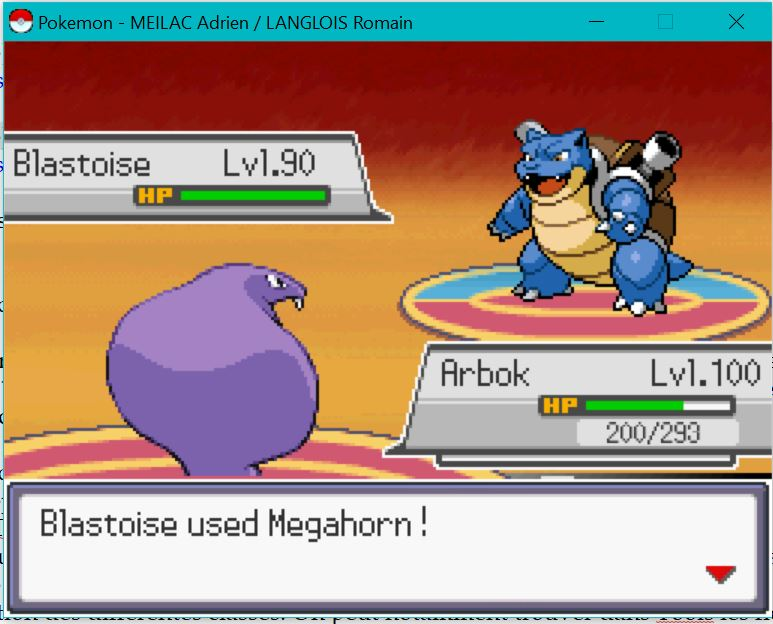
\includegraphics[scale = 0.6]{../Images/useMove.jpg}
\end{minipage}
\begin{minipage}{0.49\textwidth}
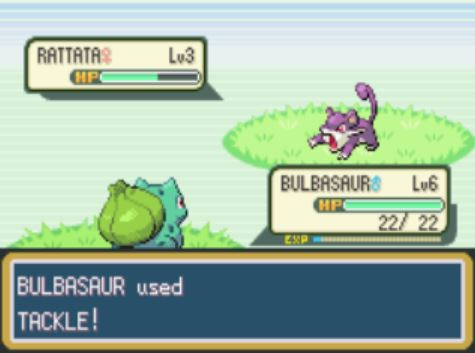
\includegraphics[scale = 0.84]{../Images/vrai_jeu_useMove.jpg}
\end{minipage}
\caption{Joueur sur la carte Pokémon}
\end{figure}

Certains des Pokemon meurent ou terrassent leur adversaire en un seul tour. C'est un choix volontaire de notre part, nous avons pensé que la démonstration serait plus fluide s'il y avait possibilité d'observer directement les conséquences d'une victoire ou d'une défaite. Ces paramètres sont modifiables dans le fichier Player\_Pokemon.txt.\\

Le pokémon sélectionné par défaut, Nidorina, possède approximativement les stats de son adversaire. Le Pokemon Arbok a été configuré avec des statistiques largement surévalué pour tester les cas de victoires et les autres Pokemon ont des statistiques largement sous évalué pour tester les cas d'échec.  

Dans le cas d'une victoire, le Pokémon vainqueur reçoit des points d'expérience (exp) dans une fenêtre contextuelle, puis le joueur revient sur la map. Dans le cas où Pokemon du joueur est terrassé, ce dernier se voit contraint de sélectionner un autre Pokemon dans le menu de dressage pour pouvoir continuer le combat. Si tous les Pokemon décèdent, une boite de dialogue Game Over apparait, il convient alors de fermer le jeu pour le relancer.

\subsection{La carte du jeu}

\begin{figure}[!h]
\begin{minipage}{0.49\textwidth}
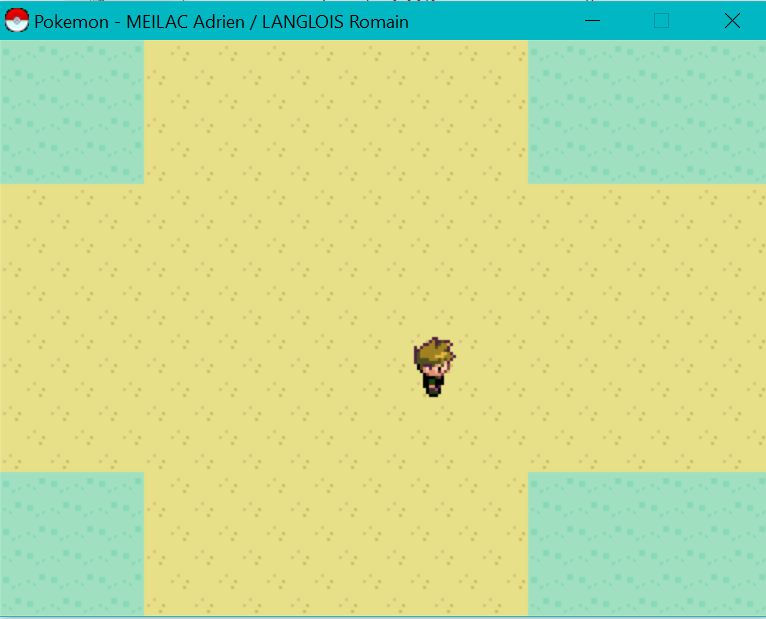
\includegraphics[scale = 0.6]{../Images/map.jpg}
\end{minipage}
\begin{minipage}{0.49\textwidth}
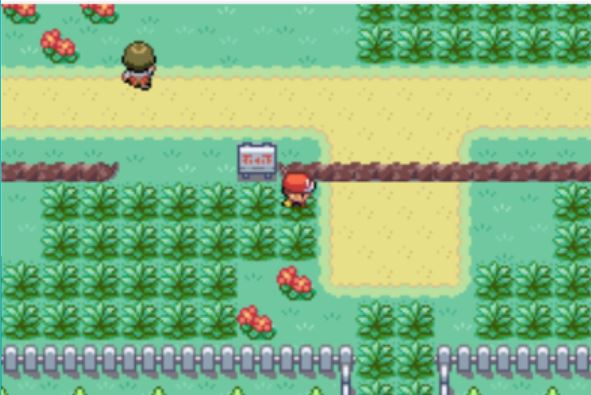
\includegraphics[scale = 0.84]{../Images/vrai_jeu_map.jpg}
\end{minipage}
\caption{Joueur sur la carte Pokémon}
\end{figure}


Le joueur est également libre de se déplacer sur la map quand il n'est pas en combat. La pression de la touche Espace lui permet d'afficher un menu. Il peut par exemple afficher ses différents Pokemon disponibles ou alors revenir sur la map à l'aide du bouton Exit. Une courte description de chaque option est également disponible.


\begin{figure}[!h]
\begin{minipage}{0.49\textwidth}
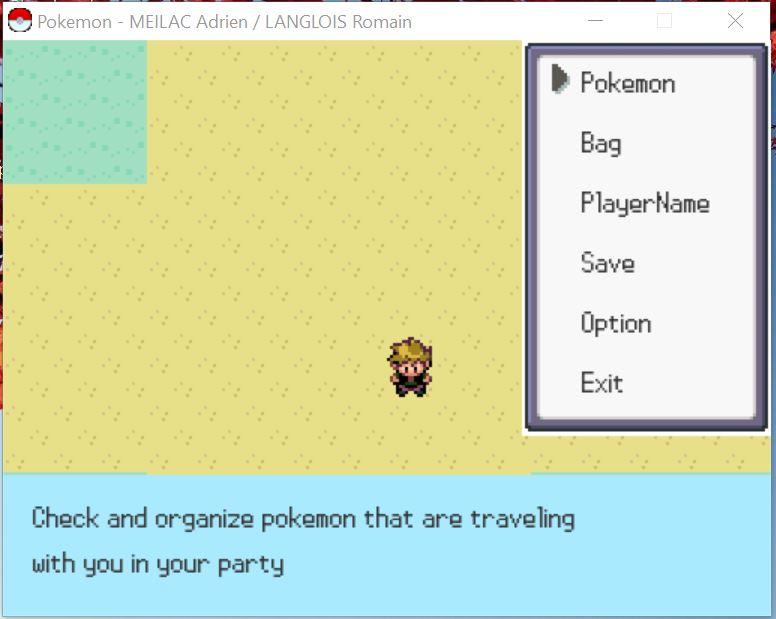
\includegraphics[scale = 0.6]{../Images/fieldMenu.jpg}
\end{minipage}
\begin{minipage}{0.49\textwidth}
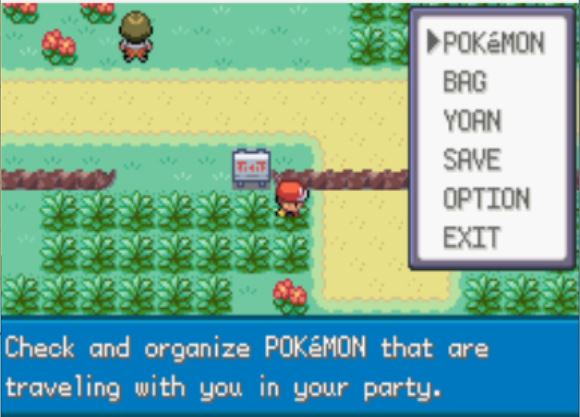
\includegraphics[scale = 0.84]{../Images/vrai_jeu_fieldMenu.jpg}
\end{minipage}
\caption{Menu sur le terrain}
\end{figure}

Nous n'avons pas réalisé l'inventaire ni les autres options de ce menu du fait d'un manque de temps, le code existant ayant déjà nécessité beaucoup de lignes, mais nous disposons désormais de tous les outils nécessaires pour réaliser ces améliorations. Pour la même raison, nous n'avons laissé qu'une seule couche d'arrière-plan sur la map et n'avons pas eu le temps de gérer les déplacements de la carte, ni la liaison entre la carte et des lieux stockés dans les données, ni l'affichage des bâtiments.
